\documentclass[11pt, a4paper]{report}

% --- Packages for Formatting ---
\usepackage[utf8]{inputenc}
\usepackage[T1]{fontenc}
\usepackage{tikz} 
\usepackage{colortbl}
\usepackage{amsmath}
\usepackage{geometry}
\geometry{
    left=0.8in,    % Space for binding/stapling
    right=0.6in,   % Narrower right margin
    top=0.7in,     % Reduce top space
    bottom=0.7in   % Reduce bottom space
}
\usepackage{setspace}
\onehalfspacing             % 1.5 spacing is standard for reports
\usepackage{titlesec}       % To customize chapter titles
\usepackage{booktabs}       % For professional looking tables
\usepackage{tabularx}       % For tables that auto-fit page width
\usepackage{graphicx}       % For images
\usepackage{float}          % To control table/figure placement
\usepackage{enumitem}   % To customize lists
\usepackage{hyperref}       % For clickable links
\geometry{margin=0.5in} 

% --- Chapter Title Formatting ---
\titleformat{\chapter}[display]
  {\normalfont\bfseries}{}{0pt}{\Huge}

\begin{document}

% ===================================================================
% CHAPTER 6
% ===================================================================

\chapter{Classification of Goods and Services Produced by Ferrari}

\section{Veblen Goods and Inelastic Demand}
From a microeconomic perspective, Ferrari vehicles defy standard demand curves. They are classified as \textbf{Veblen Goods}: luxury commodities for which the quantity demanded increases as the price increases, due to an exclusive nature and status appeal.

\begin{itemize}
    \item \textbf{Specialty Classification:} In marketing terms, these are specialty goods where the cross-price elasticity of demand is low; consumers will not accept substitutes (e.g., a Porsche) purely based on price differentials.
    \item \textbf{Signaling Utility:} Consumption is driven not only by functional utility (transportation) but by signaling utility—the ability to signal wealth and social standing to others.
\end{itemize}

\section{Durable Goods and Asset Economics}
Vehicles are traditionally treated as durable goods subject to depreciation. However, Ferrari’s limited production strategy alters the intertemporal choice model for buyers:

\begin{itemize}
    \item \textbf{Store of Value:} Unlike standard vehicles, specific Ferrari models (particularly the \textit{Icona} series or limited V12s) function as investment assets. The expected resale value often exceeds the initial purchase price, creating a negative depreciation rate.
    \item \textbf{Temporal Utility:} The ``flow of services'' includes driving pleasure and access to an exclusive club. Buyers calculate the Net Present Value (NPV) of ownership by factoring in maintenance costs against the high probability of asset appreciation.
\end{itemize}


\begin{figure}[h!]
    \centering
    \begin{tikzpicture}[scale=1.0]
        % Axes
        \draw[->] (0,0) -- (8,0) node[right] {Quantity ($Q$)};
        \draw[->] (0,0) -- (0,6) node[above] {Price ($P$)};
        
        % Vertical Supply Curve (Artificial Scarcity)
        \draw[thick, blue] (3,0) -- (3,5.5) node[above] {$S_{fixed}$};
        \draw[dashed] (3,0) -- (3,-0.5) node[below] {$Q_{capped}$};
        
        % Demand Curve (Standard)
        \draw[thick, red] (1,5) -- (6,1) node[right] {$D_{standard}$};
        
        % Demand Curve (Veblen/High Brand Equity)
        \draw[thick, red, dashed] (2,5.5) -- (7,1.5) node[right] {$D_{luxury}$};
        
        % Equilibrium Points
        \filldraw[black] (3,3.4) circle (2pt) node[anchor=south west] {$E_1$};
        \filldraw[black] (3,4.7) circle (2pt) node[anchor=south west] {$E_2$};
        
        % Price dotted lines
        \draw[dotted] (0,3.4) -- (3,3.4);
        \draw[dotted] (0,4.7) -- (3,4.7);
        
        % Labels
        \node[left] at (0,3.4) {$P_{market}$};
        \node[left] at (0,4.7) {$P_{ferrari}$};
        
        % Scarcity Premium Brace
        \draw[decorate,decoration={brace,amplitude=5pt}] (0.2,3.4) -- (0.2,4.7) 
            node[midway, left=8pt] {\footnotesize Scarcity Premium};
            
    \end{tikzpicture}
    \caption{\textbf{The Economics of Artificial Scarcity.} Unlike standard manufacturers, Ferrari fixes Supply $S_{\text{fixed}}$ perfectly vertical. As Brand Equity shifts Demand from $D_{\text{standard}}$  to $D_{\text{luxury}}$, the price increases ($P_{ferrari}$) without necessitating an increase in production volume.}
    \label{fig:scarcity_curve}
\end{figure}


\section{The Service Ecosystem (Ferrari Classiche \& Aftersales)}
Ferrari has shifted from a pure manufacturing model to a service-dominant logic to capture lifetime value.

\begin{itemize}
    \item \textbf{Information Asymmetry Reduction:} Programs like \textit{Ferrari Classiche} (certification of authenticity) reduce information asymmetry in the secondary market, artificially inflating the value of vintage models.
    \item \textbf{Maintenance as Retention:} The ``7-Year Genuine Maintenance'' program internalizes the cost of ownership, reducing the perceived barrier to entry while ensuring dealer network retention.
\end{itemize}

% --- TABLE 6.1 ---
\begin{table}[H]
    \centering
    \caption{Economic Classification of Ferrari’s Portfolio}
    \label{tab:ferrari_portfolio}
    \vspace{0.3cm}
    % The 'X' column type automatically wraps text to fit the width
    \begin{tabularx}{\textwidth}{@{} l >{\raggedright\arraybackslash}X >{\raggedright\arraybackslash}X @{}}
        \toprule
        \textbf{Category} & \textbf{Examples} & \textbf{Economic/Marketing Relevance} \\
        \midrule
        \textbf{Core Goods (Veblen)} & Icona Series (Daytona SP3), Hypercars (LaFerrari) & \textbf{Artificial Scarcity:} Supply is strictly capped below demand to maintain high equilibrium prices and exclusivity. \\
        \addlinespace
        \textbf{Production Goods} & Roma, Purosangue (SUV), 296 GTB & \textbf{Revenue Drivers:} Higher volume models that fund R\&D. These rely on high Willingness To Pay (WTP) and brand differentiation. \\
        \addlinespace
        \textbf{Complementary Goods} & Merchandise, Licensing (Watches, Apparel) & \textbf{Brand Extension:} Low barrier-to-entry goods that extract consumer surplus from aspirational fans who cannot afford the core product. \\
        \addlinespace
        \textbf{Services} & Ferrari Classiche, Corse Clienti & \textbf{Lock-in Effect:} Creates high switching costs. Owners are ``locked'' into the ecosystem through track days and certification services. \\
        \addlinespace
        \textbf{Digital Goods} & Esports Team, MyFerrari App & \textbf{Data Monopolization:} Collects user data for CRM personalization and engages the next generation of buyers (Gen Z). \\
        \bottomrule
    \end{tabularx}
\end{table}


% --- INSERT THIS IN CHAPTER 6 (New Section Idea: 6.4 Comparative Advantage) ---

\section{Benchmarking: Automaker vs. Luxury House}
To understand Ferrari's economic classification, one must compare its operating margins to standard automakers. Ferrari trades at multiples closer to Hermès or LVMH than to Volkswagen or Ford.

\begin{table}[H]
    \centering
    \caption{Operational Efficiency Comparison (Illustrative 2023/2024 Data)}
    \label{tab:competitors}
    \begin{tabularx}{\textwidth}{l c c X}
        \toprule
        \textbf{Company} & \textbf{EBIT Margin} & \textbf{Avg. Selling Price} & \textbf{Economic Classification} \\
        \midrule
        \textbf{Ferrari (RACE)} & \textbf{$\approx$ 27\%} & \textbf{$>$ \$350k} & \textbf{Veblen / Ultra-Luxury} \\
        Porsche & $\approx$ 18\% & $\approx$ \$110k & Premium Luxury \\
        Mercedes-Benz & $\approx$ 12\% & $\approx$ \$70k & Premium Consumer \\
        Ford / GM & $\approx$ 6-8\% & $\approx$ \$50k & Mass Market Durable \\
        \bottomrule
    \end{tabularx}
    \vspace{0.2cm}
    \small{\textit{Note: Ferrari's significantly higher EBIT margin indicates pricing power derived from brand equity rather than economies of scale.}}
\end{table}




% ===================================================================
% CHAPTER 7
% ===================================================================

\chapter{Ferrari's Marketing Methods and Promotional Strategies}

\section{The Economics of Artificial Scarcity}
Ferrari’s marketing logic is grounded in the economic principle of \textbf{Artificial Scarcity}. By deliberately limiting production volumes (historically capping units sold per year despite rising demand), Ferrari shifts the supply curve leftward. This ensures that:

\begin{enumerate}
    \item \textbf{Price Maker Status:} The company retains strong pricing power.
    \item \textbf{Excess Demand:} Long waiting lists create social proof and maintain high residual values for existing owners.
\end{enumerate}

\section{The Promotional Mix}
Ferrari does not utilize traditional ``push'' advertising. Instead, it relies on a ``pull'' strategy driven by heritage and performance.

\begin{itemize}
    \item \textbf{Public Relations (The Formula 1 Halo):} The Scuderia Ferrari F1 team is the primary marketing engine. It serves as a global R\&D billboard. The high fixed costs of F1 are justified by the ``Halo Effect,'' where racing victories validate the technological superiority of road cars.
    \item \textbf{Experiential Marketing \& Clustering:} Events like the \textit{Ferrari Cavalcade} create network effects. By gathering owners together, Ferrari strengthens the social capital associated with the brand, making the ``club'' harder to leave.
    \item \textbf{Personal Selling:} The sales process resembles private banking more than car retailing. Dealerships act as gatekeepers, allocating limited edition allocations (options to buy) only to top-tier clients, incentivizing loyalty.

\begin{figure}[H]
    \centering
    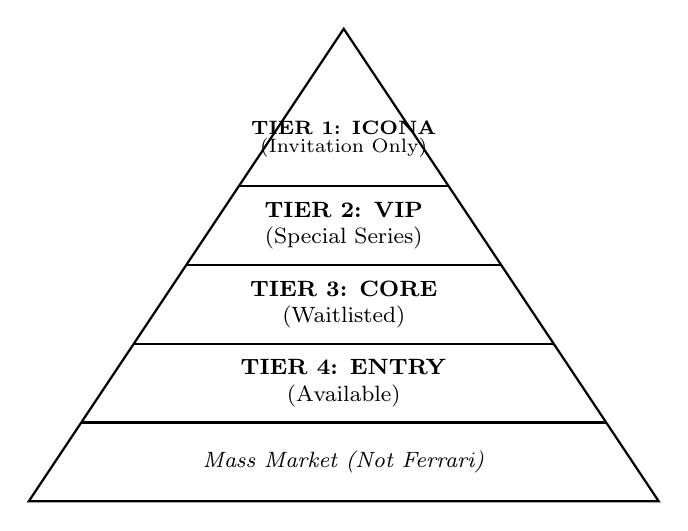
\begin{tikzpicture}
        % Define the coordinates for the pyramid
        \coordinate (A) at (-4,0);
        \coordinate (B) at (4,0);
        \coordinate (C) at (0,6);
        
        % Draw the big triangle
        \draw[thick] (A) -- (B) -- (C) -- cycle;
        
        % Draw horizontal lines to slice the pyramid
        \draw[thick] (-3.33, 1) -- (3.33, 1);
        \draw[thick] (-2.66, 2) -- (2.66, 2);
        \draw[thick] (-2, 3) -- (2, 3);
        \draw[thick] (-1.33, 4) -- (1.33, 4);
        
        % Add Text Labels (Centered)
        
        % Top Tier
        % Top Tier (Icona) - Adjusted to fit better
        \node[align=center, font=\scriptsize] at (0, 4.6) {\textbf{TIER 1: ICONA}\\[-0.5ex] (Invitation Only)};
        
        % Tier 2
        \node[align=center, font=\footnotesize] at (0, 3.5) {\textbf{TIER 2: VIP}\\(Special Series)};
        
        % Tier 3
        \node[align=center, font=\footnotesize] at (0, 2.5) {\textbf{TIER 3: CORE}\\(Waitlisted)};
        
        % Tier 4
        \node[align=center, font=\footnotesize] at (0, 1.5) {\textbf{TIER 4: ENTRY}\\(Available)};
        
        % Base
        \node[align=center, font=\footnotesize] at (0, 0.5) {\textit{Mass Market (Not Ferrari)}};
        
    \end{tikzpicture}
    \caption{\textbf{The Ferrari Ladder of Exclusivity.} Ferrari utilizes a "Conquest to Icona" funnel. Allocation of high-margin limited editions (Tier 1) acts as a reward mechanism.}
    \label{fig:client_pyramid_visual}
\end{figure}



    
    \item \textbf{Sponsorships (Co-Branding):} Partnerships with brands like Richard Mille or Bang \& Olufsen are not just revenue sources; they are signaling mechanisms that reinforce the ``high-performance luxury'' position through association.
\end{itemize}


\section{Integrated Marketing Communications (IMC)}

For Ferrari, IMC ensures that the brand narrative remains consistent across all touchpoints. Unlike mass-market manufacturers that prioritize "reach" (viewership numbers), Ferrari prioritizes "resonance" (depth of engagement). The strategy rests on two economic pillars:

\subsection{The "Silent" Marketing Paradox}
Ferrari notably avoids mass media advertising (TV commercials, billboards). In economic signaling theory, this is a strategic choice. High-volume advertising is often a signal of elastic demand (the need to chase buyers). By \textit{not} advertising, Ferrari signals that demand already exceeds supply. The brand relies on "earned media" (viral social media content, journalist reviews) which has a marginal cost of zero but high credibility.

\subsection{The Digital "Atelier" Strategy}
Ferrari has digitized the "Personal Selling" experience to capture the younger demographic (Gen Z/Millennials). The \textit{MyFerrari} application acts as a "digital ledger," tracking the vehicle's history, service needs, and exclusive event invitations. This reduces the transaction costs of ownership and keeps the client perpetually connected to the dealer network, increasing the Lifetime Value (LTV) of the customer.

\begin{figure}[H]
    \centering
    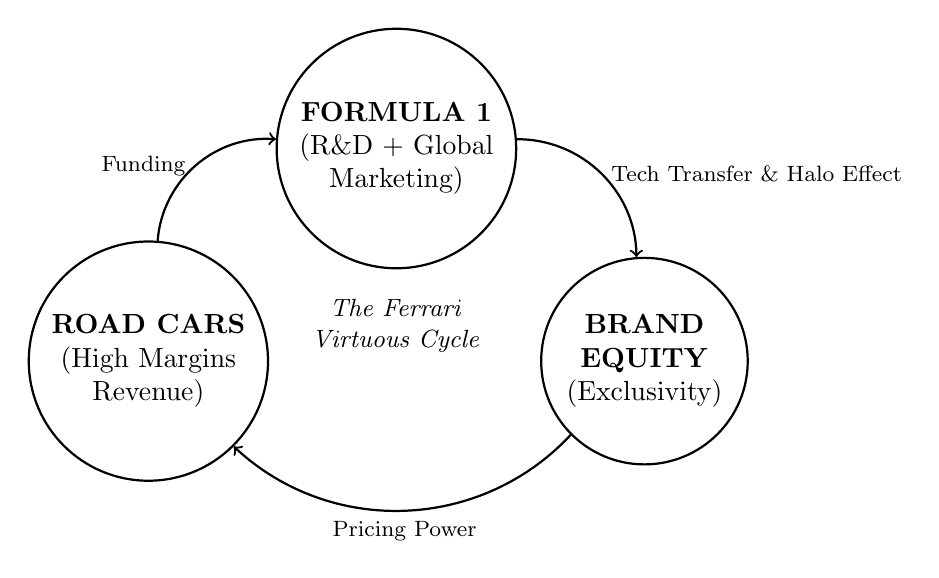
\begin{tikzpicture}[scale=0.9]
        % Nodes
        \node[draw, circle, align=center, minimum size=2.5cm, thick] (F1) at (0, 3) {\textbf{FORMULA 1} \\ (R\&D + Global \\ Marketing)};
        \node[draw, circle, align=center, minimum size=2.5cm, thick] (Brand) at (3.5, 0) {\textbf{BRAND} \\ \textbf{EQUITY} \\ (Exclusivity)};
        \node[draw, circle, align=center, minimum size=2.5cm, thick] (Road) at (-3.5, 0) {\textbf{ROAD CARS} \\ (High Margins \\ Revenue)};
        
        % Arrows
        \draw[->, thick, bend left=45] (F1) to node[right, font=\footnotesize] {Tech Transfer \& Halo Effect} (Brand);
        \draw[->, thick, bend left=45] (Brand) to node[below, font=\footnotesize] {Pricing Power} (Road);
        \draw[->, thick, bend left=45] (Road) to node[left, font=\footnotesize] {Funding} (F1);
        
        % Center Label
        \node[align=center, font=\small] at (0,0.5) {\textit{The Ferrari} \\ \textit{Virtuous Cycle}};
        
    \end{tikzpicture}
    \caption{\textbf{The Ferrari "Virtuous Cycle."} Marketing spending is concentrated in Formula 1. Success on track creates Brand Equity, which allows for high pricing on Road Cars. The profits from Road Cars are then reinvested into F1, completing the cycle.}
    \label{fig:virtuous_cycle}
\end{figure}
\end{document}
